\jxhj{%教学后记
	}
\skrq{%授课日期
	2017年4月18日 4-5节}
\ktmq{%课题名称
	 坐标系旋转2}
\jxmb{%教学目标,每行前面要加 \item
	\item 掌握Fanuc上的坐标系旋转指令;
	\item 掌握Siemens上的坐标系旋转指令;
	\item 会使用旋转指令编程。 }
\jxzd{%教学重点,每行前面要加 \item
	\item Fanuc上的坐标系旋转指令;
	\item Siemens上的坐标系旋转指令。 }
\jxnd{%教学难点,每行前面要加 \item
	\item 使用旋转指令编程。 }
\jjff{%教学方法
	通过讲述、举例、演示法来说明;}

\makeshouye %制作教案首页

%%%%教学内容
\subsection{组织教学}
\begin{enumerate}[\hspace{2em}1、]
	\item 集中学生注意力;
	\item 清查学生人数;
	\item 维持课堂纪律;
\end{enumerate}
\subsection{复习导入及主要内容}
\begin{enumerate}[\hspace{2em}1、]
\item 几种坐标系;
\item Fanuc上的局部坐标系;
\item Siemens上的局部坐标系;
\item 应用实例;
\end{enumerate}


\subsection{教学内容及过程}

\subsubsection{旋转可用于以下几种情况}
\begin{itemize}
\item 编程轮廓与工件安装面成一定角度。
\item 有多个旋转的相同轮廓。
\item 同一轮廓上有多个旋转的要素。
\item 其它简化程序的地方。
\end{itemize}

\subsubsection{要素及原理}
\paragraph{旋转指令的要素}
\begin{itemize}
\item 旋转平面
\item 旋转中心
\item 旋转角度
\end{itemize}
\paragraph{原理}
在CNC内部对目标点进行转换(我们不用管它)
$$X’=X*COSA+Y*SINA$$
$$Y’=Y*COSA-X*SINA$$

上图中的A为-45度(即从$X------X’$的方向)
\subsubsection{Fanuc指令格式}
G17\\
G18 G68 α\_ β\_ R\_; 坐标系旋转开始\\
G19\\
:                  坐标系旋转模式 \\
:                  ( 坐标系被旋转 )\\
G69;                坐标系旋转取消模式\\
说明:\\
G17(G18或G19): 选择包含有被旋转图形的平面\\
α\_β\_ :         对应当前平面指令(G17,G18或G19)中的两个轴的绝对指令。\\
此指令指定了G68后面指定旋转中心的坐标。\\
R\_    :         正值为逆时针方向的角度位移。参数5400Bit0指定角度位移是绝对值位移或者由G码(G90或G91)来决定绝对值或相对值。\\
最小输入增量: 0.001度\\
有效数据范围: -360.000~360.000\\
注意事项:
\begin{enumerate}[A、]
	\item α\_β\_省略时,默认的旋转中心为刀具当前位置。
\item 程序的开头要加上G69安全注消指令。
\item 在坐标系旋转后,执行刀具半径补偿、刀具长度补偿、刀具偏置和其它补偿等,要在坐标系旋转取消前取消补偿。
\item 在坐标系旋转中,不得执行与坐标系有关的指令。如:G27、G28、G29、G30,G52-G59。
\item  坐标系旋转取消(G69)后的第一个指令必须用绝对值编程。用增量值则不能正确的执行。
\item 坐标系G68后的第一个指令应用绝对值编程,用增量值编程,则    会以刀具当前为中心进行第二次旋转,如图\ref{旋转5}所示:
\begin{figure}
	\centering	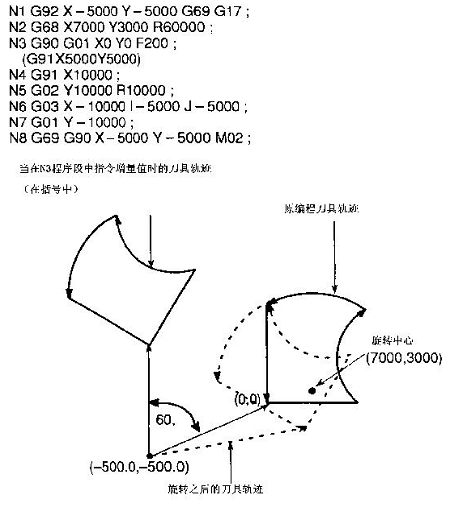
\includegraphics[width=0.8\textwidth]{images/7-1}
	\caption{旋转5} \label{旋转5}
\end{figure}
\item 有多个旋转时,旋转中的终点应与下一个旋转的启点重合。或者另外增加路径定位。
\end{enumerate}
\subsubsection{Sienes指令格式}
功能:在当前的平面G17或G18或G19中执行旋转,值为 RPL=\_,单位为度。\\
编程:    ROT RPL=\_  可编程旋转,删除以前的偏移,旋转,比例系数和镜像指令。\\
AROT RPL=\_; 可编程旋转,附加于当前的指令\\
ROT    没有设定值:删除以前的偏移,旋转,比例系数和镜象\\
ROT/AROT指令要求一个独立的程序段。

注意:旋转中心始终在工件坐标系原点\\
工件坐标系原点可以通过TRANS X\_ Y\_ 进行平移。\\

\subsubsection{加工实例}
在数控机床上加工如图\ref{坐标系旋转3}所示的零件,完成加工工艺及加工程序的编写:
\begin{figure}
	\centering	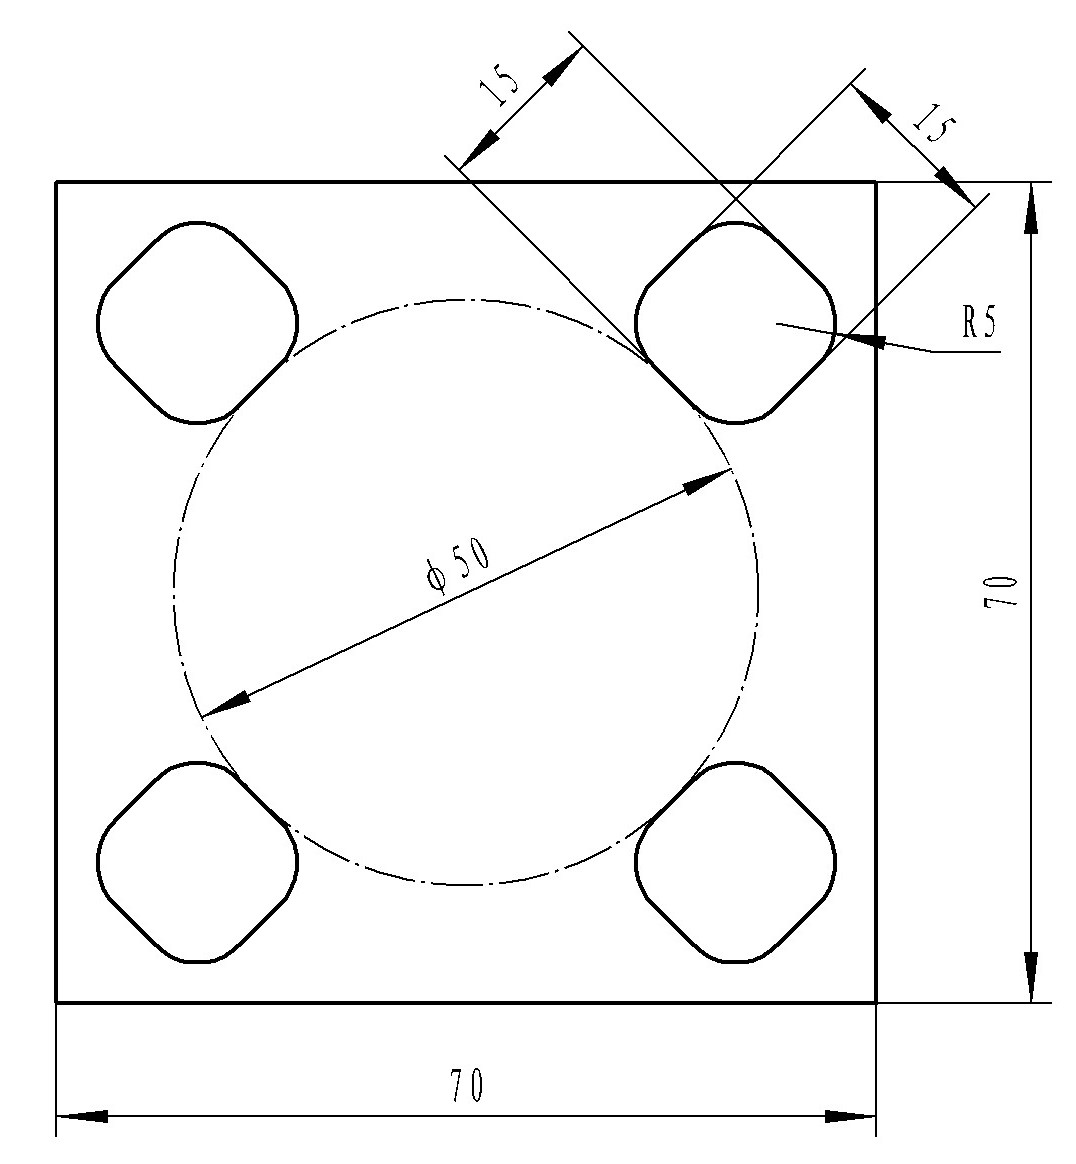
\includegraphics[width=0.8\textwidth]{images/7-2.jpg}
	\caption{坐标系旋转3} \label{坐标系旋转3}
\end{figure}
参考程序:

\begin{lstlisting}
02
G54G17G40G49G90
M3S500
G43H1G1Z100.F2000;
G1X40.Y40.
Z5.0
Z0F2000
G68X0Y0R45.
M98P221
G69
\end{lstlisting}


\subsection{课堂小结}
\begin{enumerate}[1、]
	\item 旋转可应用场合;
	\item 要素及原理;
	\item Fanuc旋转指令格式;
	\item Sienes旋转指令格式;
	\item 编程实例。
\end{enumerate}

\vfill
\subsection{布置作业}
\begin{enumerate}[1、]
	\item 综合习题一。 
\end{enumerate}
\vfill